%!TEX program = xelatex

\documentclass[compress]{beamer}
%--------------------------------------------------------------------------
% Common packages
%--------------------------------------------------------------------------

\definecolor{links}{HTML}{663000}
\hypersetup{colorlinks,linkcolor=,urlcolor=links}

\usepackage[english]{babel}
\usepackage{pgfpages} % required for notes on second screen
\usepackage{graphicx}

\usepackage{pdfpcnotes}

\usepackage{multicol}

\usepackage{tabularx,ragged2e}
\usepackage{booktabs}

\setlength{\emergencystretch}{3em}  % prevent overfull lines
\providecommand{\tightlist}{%
  \setlength{\itemsep}{0pt}\setlength{\parskip}{0pt}}


\usetheme{hri}

% Display the navigation bullet even without subsections
\usepackage{remreset}% tiny package containing just the \@removefromreset command
\makeatletter
\@removefromreset{subsection}{section}
\makeatother
\setcounter{subsection}{1}

\makeatletter
\let\beamer@writeslidentry@miniframeson=\beamer@writeslidentry
\def\beamer@writeslidentry@miniframesoff{%
  \expandafter\beamer@ifempty\expandafter{\beamer@framestartpage}{}% does not happen normally
  {%else
    % removed \addtocontents commands
    \clearpage\beamer@notesactions%
  }
}
\newcommand*{\miniframeson}{\let\beamer@writeslidentry=\beamer@writeslidentry@miniframeson}
\newcommand*{\miniframesoff}{\let\beamer@writeslidentry=\beamer@writeslidentry@miniframesoff}
\makeatother



\newcommand{\source}[2]{{\tiny\it Source: \href{#1}{#2}}}

\usepackage[normalem]{ulem}

\usepackage{tikz}
\usetikzlibrary{intersections,arrows,shapes,calc,mindmap,backgrounds,positioning,svg.path}

\tikzset{box/.style={
            draw, 
            fill=blue!20,
            fill opacity=0.8,
            thick,
            inner sep=0pt,
            minimum size=1cm,
            transform shape
        },
        finalbox/.style={
            draw, 
            fill=orange,
            fill opacity=0.8,
            thick,
            inner sep=0pt,
            minimum size=1cm,
            transform shape
        },
        dot/.style={
            draw,
            circle,
            fill=red!20,
            inner sep=0pt,
            minimum size=1cm,
            transform shape
        },
        axis/.style={
            thick,
            gray,
            font=\small},
        every to/.style={
            >=latex,
            dashed,
            thick
        }
    }


\graphicspath{{figs/}}

\title{ROCO222 \newline Intro to Sensors and Actuators}
\subtitle{Face recognition and Integration with ROS}

\date{}
\author{Séverin Lemaignan}
\institute{Centre for Neural Systems and Robotics\\{\bf Plymouth University}}

\begin{document}

\licenseframe{github.com/severin-lemaignan/module-introduction-sensors-actuators}

\maketitle

\miniframesoff

\miniframeson


\section[Principal Component Analysis]{Face recognition: Principal Component Analysis}

\imageframe{face-recognition-challenge}

{
    \paper{\source{https://pdfs.semanticscholar.org/37de/33701dd73c89a7b410d69070085b583bfd38.pdf}{Mark
    Richardson, Principal Component Analysis}}
\begin{frame}{Principal Component Analysis}

    \only<1>{
    Principal Component Analysis (PCA) is a technique to find the sources of variance in a dataset.
    }

    \only<2>{
    \begin{center}
        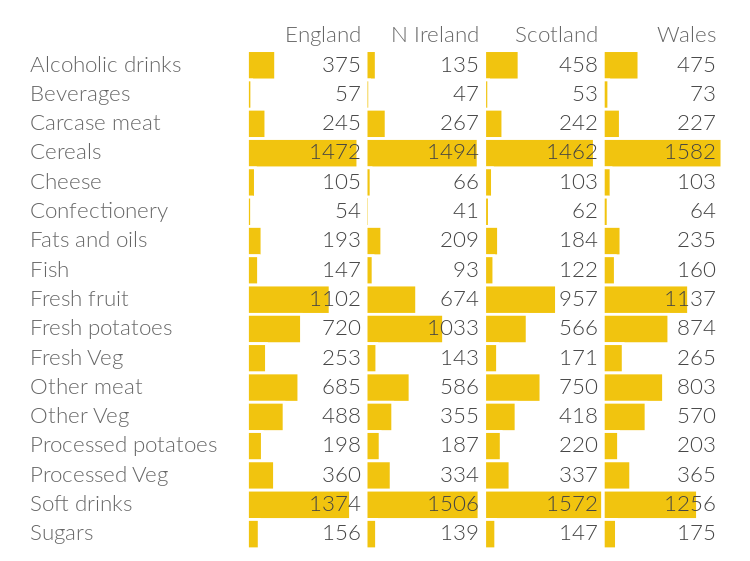
\includegraphics[width=0.8\linewidth]{pca-food-example}
    \end{center}
    }

    \only<3->{

    \begin{columns}
        \begin{column}{0.5\linewidth}
    \begin{center}
        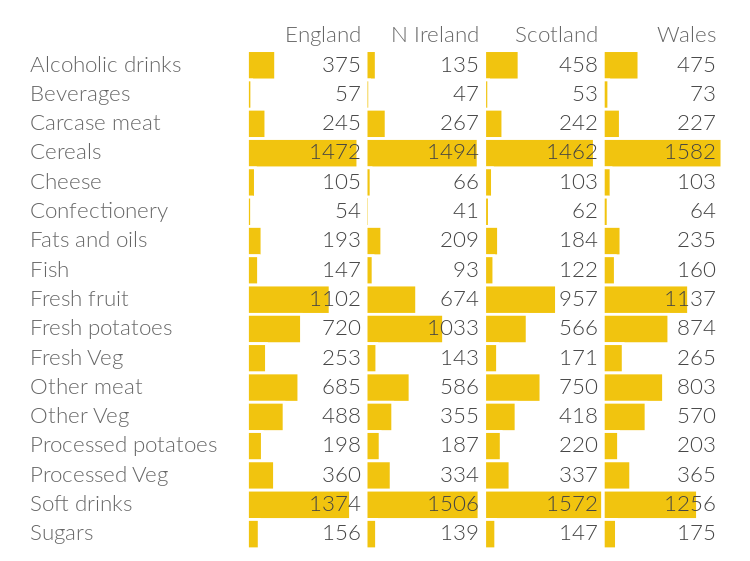
\includegraphics[width=\linewidth]{pca-food-example}
    \end{center}

        \end{column}
        \begin{column}{0.5\linewidth}
            \begin{center}
                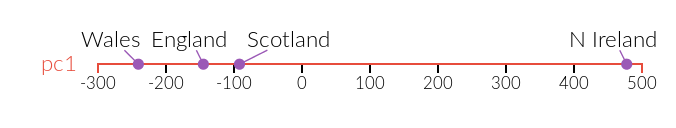
\includegraphics[width=\linewidth]{pca-food-example-1-eigenvector}

                \includegraphics<4->[width=\linewidth]{pca-food-example-2-eigenvector}

                \includegraphics<5->[width=\linewidth]{pca-food-example-load-plot}
            \end{center}
        \end{column}
    \end{columns}

    }

\end{frame}
}

\imageframe[scale=0.9, caption={Applied to handwriting}]{pca}
\videoframe{figs/cowriter.mp4?start=135}

\imageframe[scale=0.9, caption={Applied to faces}]{dataset}

{
    \paper{\source{https://github.com/bytefish/facerecognition_guide}{Philipp
    Wagner, Face Recognition with Python} (code source available as well)}

\begin{frame}{PCA Algorithm}
    Let $\mathbf{X} = \{ \mathbf{x}_{1}, \mathbf{x}_{2}, \ldots, \mathbf{x}_{n} \}$ be a vector with observations $\mathbf{x}_i \in \mathbb{R}^{d}$.

    \begin{enumerate}
        \item Compute the mean $\mu$
            \[
                \mu = \frac{1}{n} \sum_{i=1}^{n} \mathbf{x}_{i}
            \]
        \item Compute the the Covariance Matrix $S$
            \[
                S = \frac{1}{n} \sum_{i=1}^{n} (\mathbf{x}_{i} - \mu) (\mathbf{x}_{i} - \mu)^{T}
            \]
        \item Compute the eigenvalues $\lambda_{i}$ and eigenvectors $\mathbf{v}_{i}$ of $S$
            \[
                S \cdot \mathbf{v}_{i} = \lambda_{i} \mathbf{v}_{i} \text{\hspace{1em} with } i=1,2,\ldots,n
            \]
        \item Order the eigenvectors descending by their eigenvalue. The $k$
            principal components are the eigenvectors corresponding to the $k$
            largest eigenvalues.

    \end{enumerate}

\end{frame}
}


\begin{frame}[fragile]{Python code}

\begin{pythoncode}
def pca(X):

    mu = X.mean(axis=0)
    X = X - mu
    C = np.dot(X.T,X)
    eigenvalues, eigenvectors = np.linalg.eigh(C)

    # sort eigenvectors descending by their eigenvalue
    idx = np.argsort(-eigenvalues)
    eigenvalues = eigenvalues[idx]
    eigenvectors = eigenvectors[:,idx]
    return eigenvalues, eigenvectors, mu

# D: eigenvalues, W: eigenvectors, mu: mean, X: 40 X 10304 image array
D, W, mu = pca(X) 

# plot the first 16 'eigenfaces'
images = []
for i in range(16):
    image = W[:,i].reshape(X[0].shape)
    images.append(normalize(image,0,255))

subplot(title="Eigenfaces", images=images, rows=4, cols=4)

\end{pythoncode}
\end{frame}


\imageframe{dataset}
\imageframe{eigenfaces}

\begin{frame}{PCA Projection and Reconstruction}

    The $k$ principal components of an observed vector
    $\mathbf{x}\bubblemark{image}$ are then given by:

    \[
        \mathbf{y} = W^{T} (\mathbf{x} - \mu)
    \]

    where $W\bubblemark{pcabasis} = (\mathbf{v}_{1}, \mathbf{v}_{2}, \ldots, \mathbf{v}_{k})$.
    
    \bubble<1->[80][0.5][3cm]{image}{The image of a face!}
    \bubble<1->[100]{pcabasis}{The PCA basis}

\end{frame}

\imageframe[scale=0.8]{pca-projections-1}
\imageframe[scale=0.8]{pca-projections-2}
\imageframe[scale=0.8]{pca-projections-3}

\begin{frame}{PCA Projection and reconstruction}

    The $k$ principal components of an observed vector
    $\mathbf{x}\bubblemark{image}$ are then given by:

    \[
        \mathbf{y} = W^{T} (\mathbf{x} - \mu)
    \]

    where $W\bubblemark{pcabasis} = (\mathbf{v}_{1}, \mathbf{v}_{2}, \ldots, \mathbf{v}_{k})$.
    
    \bubble<1->[80][0.5][3cm]{image}{The image of a face!}
    \bubble<1->[100]{pcabasis}{The PCA basis}


    The reconstruction from the PCA basis is given by:

    \[
        \mathbf{x} = W \cdot \mathbf{y} + \mu
    \]

\end{frame}

\begin{frame}[fragile]{Python code}

\begin{pythoncode}
def project(W, X, mu=None):
    if mu is None:
        return np.dot(X,W)
    return np.dot(X - mu, W)

def reconstruct(W, Y, mu=None):
    if mu is None:
        return np.dot(Y,W.T)
    return np.dot(Y, W.T) + mu

images = []
for nb_evs in range(10, 310, 20):
    P = project(W[:,0:nb_evs], X[0].reshape(1,-1), mu)
    R = reconstruct(W[:,0:nb_evs], P, mu)

    R = R.reshape(X[0].shape)
    images.append(normalize(R,0,255))

subplot(title="Reconstruction of one face", images=images, rows=4, cols=4)
\end{pythoncode}
\end{frame}

\imageframe{one-face}

\begin{frame}{Why is it useful?}


    Original images: $dim(\mathbf{x}) = 92 \times 112 = 10304$ pixels: large number of dimensions!

    $\Rightarrow$ difficult to tell whether 2 images represent the same person
    (\ie \emph{classify} them).

    \pause

    With the PCA, we project our test image onto a PCA basis of $k$ principal
    components: $\mathbf{y} = W^{T} (\mathbf{x} - \mu)$ with $W = (\mathbf{v}_{1}, \mathbf{v}_{2}, \ldots, \mathbf{v}_{k})$.


    $dim(\mathbf{y}) = k$ is much smaller than $dim(\mathbf{x})$

    \pause

    \textbf{We effectively ``summarize'' our image into a few key values}, along
    the principal axes of variation of our dataset.

    $\Rightarrow$ these values discriminate effectively amongst our images
    
    $\Rightarrow$ \textbf{Well suited for classification!}

\end{frame}

\imageframe{reconstruction-1-eigenfaces}
\imageframe{reconstruction-10-eigenfaces}
\imageframe{reconstruction-50-eigenfaces}

\begin{frame}{}
    \begin{center}
        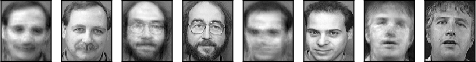
\includegraphics[width=\linewidth]{reconstruction-50-eigenfaces-top-row}

        \vspace{2em}
        Remember: these faces are reconstructed from 50 values (to be compared
        to the 10304 values required for the original photos).

        \vspace{2em}

        \pause

        PCA is often used as a \textbf{dimensionality reduction} technique (\ie a
        kind of data lossy data compression).

    \end{center}
\end{frame}


\section[Face recognition]{Face recognition}

\imageframe{face-recognition-challenge}

\imageframe[scale=0.8]{pca-projections-4}
\imageframe[scale=0.8]{pca-projections-5}
\imageframe[scale=0.8]{pca-projections-6}

\begin{frame}{Recognition}

    \begin{enumerate}
        \item \textbf{learn a model} by projecting the training set onto the PCA
            basis
        \item \textbf{project the test image} as well
        \item \textbf{find the 1-nearest neighbour}
    \end{enumerate}
\end{frame}

\begin{frame}[fragile]{Python code}


    \begin{columns}
        \begin{column}{0.5\linewidth}
\begin{minted}[fontsize=\scriptsize]{python}
def dist(p, q):
    p = np.asarray(p).flatten()
    q = np.asarray(q).flatten()
    return np.sqrt(np.sum(
                    np.power((p-q),2)
                    ))


def learn_model(X):
    D, W, mu = pca(X, nb_evs=10)
    # compute projections
    projections = []
    for xi in X:
        yi = project(W,
                   xi.reshape(1,-1), 
                   mu)
        projections.append(yi)

    return W, projections
\end{minted}

        \end{column}
        \begin{column}{0.5\linewidth}


\begin{minted}[fontsize=\scriptsize]{python}
def predict(X, W, projections):
    minDist = np.finfo('float').max
    minClass = -1
    Q = project(W, X.reshape(1,-1), mu)

    for i in range(len(projections)):
        dist = dist(projections[i], Q)
        if dist < minDist:
            minDist = dist
            faceClass = faceClasses[i]
    return faceClass


X, faceClasses = read_images()
W, projections = learn_model(X)
predict(test_image, W, projections)

\end{minted}
        \end{column}
    \end{columns}

\end{frame}

\begin{frame}{Limits of the PCA approach (Eigenfaces)}

    PCA tries to find a combination of linear features that maximizes the total
    variance (\ie the ``axes of maximum variation'').
    
    No concept of class!

\end{frame}

\imageframe[caption={Here, 10 images per class -- we only want to learn
between-class discriminant features}]{dataset}
\imageframe[caption={For instance, the PCA (wrongly) encodes the illumination}]{eigenfaces}


{
    \paper{\source{http://www.cs.jhu.edu/~hager/Public/teaching/cs461/pami97-eigenfaces.pdf}{Belhumeur, Hespanha and Kriegman, Eigenfaces vs.
    fisherfaces: Recognition using class specific linear projection}}

\begin{frame}{Limits of the PCA approach (Eigenfaces)}

    $\Rightarrow$ Linear Discriminant Analysis (LDA) (and the corresponding
    \emph{Fischerfaces})

    LDA tries to find a combination of linear features that maximizes the ratio
    of between-classes to within-classes scatter.

\end{frame}
}


\miniframesoff
\begin{frame}[plain]
    \begin{center}
        \Large
        10 min break\\[2em]
    \end{center}
\end{frame}
\miniframeson

\section[With ROS]{How to integrate that with ROS?}

\begin{frame}{Reminder: a simple image processing pipeline}

\begin{center}
\begin{tikzpicture}[
                    >=latex,
                    every edge/.style={->, draw, very thick},
                    service/.style={->, draw, very thick,dashed},
                    rosnode/.style={draw, font=\sf, node distance=0.5, rounded
                    corners, align=center, inner sep=5pt,fill=hriSec2Dark!50},
                    topic/.style={font=\tt, node distance=0.5, align=center, inner sep=5pt},
                    pic/.style={fill=none,draw=none}
                ]

    \node [rosnode] at (-4,0) (node1) {image acquisition};
    \node [rosnode] at (0,-2) (node2) {image processor};
    \node [rosnode] at (4,-4) (node3) {next processing};

        \node [topic] at (-4,-1.5) (topic3) {/image};
        \node [topic] at (-1,-3.5) (topic1) {/processed\_image};
        \path (node1) edge[bend right] (node2);
        \path (node2) edge[bend right] (node3);


    \uncover<2-> {

        \node at (-0,0) (a) {this is a \textbf{node}};
        \path[dashed] (a) edge (node1);
        \node at (-4.5,-3) (b) {this is a \textbf{topic}};
        \path[dashed] (b) edge (topic3);
    }
\end{tikzpicture}
\end{center}

\end{frame}

%\begin{frame}{Example: a simple image processing pipeline}
%
%\begin{center}
%\begin{tikzpicture}[
%                    >=latex,
%                    every edge/.style={->, draw, very thick},
%                    service/.style={->, draw, very thick,dashed},
%                    rosnode/.style={draw, font=\sf, node distance=0.5, rounded
%                    corners, align=center, inner sep=5pt,fill=hriSec2Dark!50},
%                    topic/.style={font=\tt, node distance=0.5, align=center, inner sep=5pt},
%                    pic/.style={fill=none,draw=none}
%                ]
%
%    \node [rosnode] at (-4,0) (node1) {\tt gscam};
%    \node [rosnode] at (0,-2) (node2) {\tt our\_processing};
%    \node [rosnode] at (4,-4) (node3) {\tt next\_processing};
%
%        \node [topic] at (-1.2,-0.7) (topic2) {/v4l/camera/image\_raw};
%        \node [topic] at (-2.4,-2.2) (topic3) {/image};
%        \node [topic] at (1.4,-2.7) (topic1) {/processed\_image};
%        \path (node1) edge[bend right] (node2);
%        \path (node2) edge[bend right] (node3);
%
%
%\end{tikzpicture}
%\end{center}
%
%\end{frame}


\begin{frame}[containsverbatim]{}

\begin{minted}[frame=none,
               linenos=true,
               fontsize=\footnotesize,
               numbersep=0.4em,
               xleftmargin=0.5em]{python}
import sys, cv2, rospy
from sensor_msgs.msg import Image
from cv_bridge import CvBridge

def on_image(image):
    cv_image = bridge.imgmsg_to_cv2(image, "bgr8")
    rows, cols, channels = cv_image.shape
    cv2.circle(cv_image, (cols/2, rows/2), 50, (0,0,255), -1)
    image_pub.publish(bridge.cv2_to_imgmsg(cv_image, "bgr8"))

rospy.init_node('image_processor')
bridge = CvBridge()
image_sub = rospy.Subscriber("image",Image, on_image)
image_pub = rospy.Publisher("processed_image",Image)

while not rospy.is_shutdown():
    rospy.spin()
\end{minted}

\end{frame}

\begin{frame}[fragile]{How to use this code?}

First, we need to write data onto the \texttt{/image} topic, for instance from a
webcam:

\begin{shcode}
> rosrun usb_cam usb_cam_node
\end{shcode}

\pause

Then, we run our code:

\begin{shcode}
> python image_processor.py image:=/usb_cam/image_raw
\end{shcode}

\pause

Finally, we run a 3rd node to display the image:

\begin{shcode}
> rqt_image_view image:=/processed_image
\end{shcode}

\end{frame}

\imageframe[color=black]{image_processor.png}

\section{Creating the FaceRec ROS package}

\begin{frame}[fragile]{Let's create a proper ROS package}

\begin{shcode}
> cd $HOME
> mkdir src && cd src
> catkin_create_pkg facerec rospy
\end{shcode}
\pause
\begin{shcode}
> ls facerec
CMakeLists.txt  package.xml  src
\end{shcode}

\end{frame}

\begin{frame}[fragile]{First, add some code}

\begin{shcode}
> cd facerec
> mkdir -p src/facerec && cd src/facerec
> touch __init__.py # required to create a Python module
> gedit recognition.py
\end{shcode}
\pause

Just a simple stub for a Python module:

\begin{pythoncode}
def run(dataset):
    print('Dataset: ' + dataset)
\end{pythoncode}

\end{frame}

\begin{frame}[fragile]{First, add some initial code}

Create as well an executable (our future ROS node) in \texttt{scripts/}:

\begin{shcode}
> cd ../..
> mkdir -p scripts && cd scripts
> gedit reco
\end{shcode}
\pause

\begin{pythoncode}
#! /usr/bin/env python

import facerec.reco

if __name__ == '__main__':
    facerec.reco.run("my_faces")
\end{pythoncode}

\pause

\begin{shcode}
> chmod +x reco
\end{shcode}
\end{frame}

\begin{frame}[fragile]{Configure the Python 'build'}

Because our node is written in Python, our \texttt{CMakeLists.txt} is simple:

\begin{cmakecode}
cmake_minimum_required(VERSION 2.8.3)
project(facerec)

find_package(catkin REQUIRED COMPONENTS
  rospy
)

catkin_python_setup()
catkin_package()

install(PROGRAMS
   scripts/reco
   DESTINATION ${CATKIN_PACKAGE_BIN_DESTINATION}
)

\end{cmakecode}
\end{frame}

\begin{frame}[fragile]{Configure the Python 'build'}

However, we need a \texttt{setup.py} (standard Python
    \texttt{distutils}-based packaging):

\begin{pythoncode}
from distutils.core import setup
from catkin_pkg.python_setup import generate_distutils_setup

# fetch values from package.xml
setup_args = generate_distutils_setup(
                    packages=['facerec'],
                    package_dir={'': 'src'},
                )

setup(**setup_args)
\end{pythoncode}

\end{frame}

\begin{frame}[fragile]{Install the node}

    We can now install our node:

\begin{shcode}
> cd ..
> mkdir -p build && cd build
> cmake -DCMAKE_INSTALL_PREFIX=<install prefix> ..
> make install
\end{shcode}

\pause

Assuming ROS is correctly installed, we can run our node:

\begin{shcode}
> export ROS_PACKAGE_PATH=<prefix>/share:$ROS_PACKAGE_PATH
> rosrun facerec reco
Dataset: my_faces
\end{shcode}


\end{frame}

\begin{frame}[fragile]{Image processing}
Let's update the node \texttt{reco} and the library (Python \emph{module})
    \texttt{recognition.py} to perform simple image processing:

\texttt{recognition.py}:
\begin{pythoncode}
import cv2

def run(image):
    rows, cols, channels = image.shape
    cv2.circle(image, (cols/2, rows/2), 50, (0,0,255), -1)
\end{pythoncode}
\end{frame}

\begin{frame}[fragile]{Image processing}
\texttt{reco}:
\begin{pythoncode}
#! /usr/bin/env python

import sys, rospy
from sensor_msgs.msg import Image
from cv_bridge import CvBridge

import facerec.reco

def on_image(image):
    cv_image = bridge.imgmsg_to_cv2(image, "bgr8")
    facerec.reco.run(cv_image)
    image_pub.publish(bridge.cv2_to_imgmsg(cv_image, "bgr8"))

if __name__ == '__main__':
    rospy.init_node('image_processor')
    bridge = CvBridge()
    image_sub = rospy.Subscriber("image",Image, on_image)
    image_pub = rospy.Publisher("processed_image",Image, queue_size=1)

    while not rospy.is_shutdown():
        rospy.spin()
\end{pythoncode}

\end{frame}

\begin{frame}[fragile]{To use the node}


\begin{shcode}
> rosrun usb_cam usb_cam_node
\end{shcode}


\begin{shcode}
> rosrun facerec reco image:=/usb_cam/image_raw
\end{shcode}


\begin{shcode}
> rqt_image_view image:=/processed_image
\end{shcode}

\end{frame}


\begin{frame}[plain]
    \begin{center}
        \Large
    Let's try it!
    \end{center}
\end{frame}


\begin{frame}{What are the next steps for face recognition?}

    We need to:
    \begin{itemize}
        \item acquire reference images for each of the face we want to recognise
        \item re-train the model every time we add new faces to the dataset
        \item when requested, attempt to recognise the person $\rightarrow$ ROS
            action
    \end{itemize}
\end{frame}


\begin{frame}{Possible network}

\begin{center}
\begin{tikzpicture}[
                    >=latex,
                    every edge/.style={->, draw, very thick},
                    service/.style={->, draw, very thick,dashed},
                    rosnode/.style={draw, font=\sf, node distance=0.5, rounded
                    corners, align=center, inner sep=5pt,fill=hriSec2Dark!50},
                    topic/.style={font=\tt, node distance=0.5, align=center, inner sep=5pt},
                    pic/.style={fill=none,draw=none}
                ]

    %\path[use as bounding box] (-6,1) rectangle (6,-5);
    \node [rosnode] at (0,0) (node1) {client};
    \node [rosnode] at (4,2) (node2) {facerec};
    \node [rosnode] at (8,-1) (node3) {camera};

        %\node [topic] at (1,-2) (topic1) {/topic1};
        %\node [topic] at (-1,-3) (topic2) {/topic2};
        \node [topic] at (6,-2) (topic3) {/image};
        \path (node3) edge[bend left] node[label,right] {publishes} (topic3);
        \path (node2) edge[bend right] node[label,left] {subscribes} (topic3);

        \path[->, dashed] ([xshift=-2pt]node1.north) edge[bend left] node[label,above left] {reco request} ([yshift=2pt]node2.west) ;
        \path[->, dashed] ([yshift=-2pt]node2.west) edge[bend right] node[label,below right] {reco result} ([xshift=2pt]node1.north);


\end{tikzpicture}
\end{center}

\end{frame}

\begin{frame}{Recognition logic}

    Inside \texttt{facerec}:

    \begin{itemize}
        \item when incoming request, attempt recognition
        \item if recognition fails: acquire a couple of images of that person; create a new class; re-train
        \item if recognition succeeds: add image to corresponding class; re-train
        \item if unsure: ask for confirmation
    \end{itemize}

    \pause
    \begin{center}
        \textbf{Implementation left as an exercice!}
    \end{center}
\end{frame}

\begin{frame}{}
    \begin{center}
        \Large
        That's all, folks!\\[2em]
        \normalsize
        Questions:\\
        Portland Square B316 or \url{severin.lemaignan@plymouth.ac.uk} \\[1em]

        Slides:\\
        \href{https://github.com/severin-lemaignan/module-introduction-sensors-actuators}{\small
        github.com/severin-lemaignan/module-introduction-sensors-actuators}


    \end{center}
\end{frame}



\end{document}
